\documentclass[11pt,a4paper]{article}

\usepackage[utf8]{inputenc}
\usepackage[T1]{fontenc}
\usepackage[brazilian,provide=*]{babel}
\usepackage[margin=2.5cm]{geometry}
\usepackage{xcolor}
\usepackage{hyperref}
\usepackage{longtable}
\usepackage{booktabs}
\usepackage{array}
\usepackage{tikz}
\usepackage{listings}
\usepackage{enumitem}
\usepackage{fancyhdr}
\usepackage{titlesec}
\usepackage{parskip}
\usetikzlibrary{shapes.geometric, arrows.meta, positioning, calc, fit}

\definecolor{primaria}{HTML}{1F2933}
\definecolor{destaque}{HTML}{3B82F6}
\definecolor{cinzaclaro}{HTML}{F4F6F8}

\hypersetup{
    colorlinks=true,
    linkcolor=destaque,
    urlcolor=destaque,
    citecolor=destaque,
    pdftitle={rag-chat-node - Documento de Engenharia de Software},
    pdfauthor={Bruno Silveira}
}

\titleformat{\section}{\Large\bfseries\color{primaria}}{\thesection}{1em}{}
\titleformat{\subsection}{\large\bfseries\color{primaria}}{\thesubsection}{1em}{}
\titleformat{\subsubsection}{\normalsize\bfseries\color{primaria}}{\thesubsubsection}{1em}{}

\pagestyle{fancy}
\fancyhf{}
\fancyhead[L]{\small rag-chat-node -- Documento de Engenharia de Software}
\fancyhead[R]{\small\thepage}
\renewcommand{\headrulewidth}{0.4pt}

\lstset{
    basicstyle=\ttfamily\small,
    breaklines=true,
    frame=single,
    backgroundcolor=\color{cinzaclaro},
    columns=fullflexible,
    literate=
        {á}{{\'a}}1 {à}{{\`a}}1 {â}{{\^a}}1 {ã}{{\~a}}1
        {é}{{\'e}}1 {ê}{{\^e}}1
        {í}{{\'i}}1
        {ó}{{\'o}}1 {ô}{{\^o}}1 {õ}{{\~o}}1
        {ú}{{\'u}}1 {ü}{{\"u}}1
        {ç}{{\c c}}1
        {Á}{{\'A}}1 {É}{{\'E}}1 {Í}{{\'I}}1 {Ó}{{\'O}}1 {Ú}{{\'U}}1
        {Ã}{{\~A}}1 {Õ}{{\~O}}1 {Ç}{{\c C}}1
}

\begin{document}

% ---------------------------------------------------------------- CAPA
\begin{titlepage}
    \centering
    \vspace*{2cm}
    {\Huge\bfseries\color{primaria} rag-chat-node}\\[0.5cm]
    {\Large API REST de Chat RAG (Retrieval-Augmented Generation) com Claude}\\[2cm]
    {\large Documento de Engenharia de Software}\\[0.3cm]
    {\large Levantamento de Requisitos, Casos de Uso, Arquitetura e Plano de Testes}\\[3cm]

    
\begin{tikzpicture}
        \draw[destaque, line width=1.5pt] (0,0) -- (10,0);
    \end{tikzpicture}

    \vspace{3cm}
    {\large Projeto de portfólio pessoal}\\[0.2cm]
    {\large Autor: Bruno Silveira}\\[2cm]

    \vfill
    {\large \today}
\end{titlepage}

\tableofcontents
\newpage

% ================================================================ 1
\section{Introdução}

\subsection{Contexto e objetivo}

O \textbf{rag-chat-node} é uma API REST desenvolvida como projeto de portfólio para
demonstrar, na prática, a construção de um pipeline de \emph{Retrieval-Augmented
Generation} (RAG) sobre Node.js/TypeScript: ingestão de documentos textuais, divisão
em pedaços (\emph{chunking}), geração de \emph{embeddings}, recuperação por
similaridade semântica e geração de resposta em linguagem natural com um modelo de
linguagem (Claude, da Anthropic).

O objetivo deste documento é registrar, de forma formal, o processo de engenharia de
software aplicado ao projeto: o levantamento de requisitos, a especificação dos casos
de uso, as decisões arquiteturais tomadas (registradas como ADRs -- \emph{Architecture
Decision Records}) e o plano de testes utilizado para validar o sistema.

\subsection{Escopo}

O escopo da API compreende:

\begin{itemize}[leftmargin=1.5cm]
    \item Ingestão de documentos textuais, com chunking automático e geração de
          embeddings locais (sem custo de API externa);
    \item Listagem dos documentos já ingeridos;
    \item Perguntas e respostas em linguagem natural, fundamentadas no conteúdo dos
          documentos ingeridos (RAG), com o Claude gerando a resposta final;
    \item Motor de resposta heurístico de fallback, para uso sem chave de API paga;
    \item Histórico consultável de perguntas e respostas;
    \item Documentação interativa da própria API via OpenAPI/Swagger UI.
\end{itemize}

Está fora do escopo desta versão: autenticação/autorização de usuários, persistência
em banco de dados (armazenamento é em memória) e upload de arquivos binários (PDF,
DOCX) -- apenas texto puro é aceito.

\subsection{Tecnologias utilizadas}

\begin{center}
\begin{tabular}{ll}
\toprule
\textbf{Camada} & \textbf{Tecnologia} \\
\midrule
Runtime & Node.js 20 (LTS) \\
Linguagem & TypeScript (\texttt{strict}) \\
Framework HTTP & Express \\
Validação & Zod \\
LLM & Anthropic Claude API (\texttt{@anthropic-ai/sdk}) \\
Embeddings & Modelo local via \texttt{@xenova/transformers} (\texttt{all-MiniLM-L6-v2}) \\
Vector store & Em memória (array + similaridade de cosseno) \\
Documentação de API & OpenAPI 3.0 + Swagger UI \\
Testes & Vitest + Supertest \\
Containerização & Docker + Docker Compose \\
Versionamento & Git (Git Flow) + Conventional Commits \\
\bottomrule
\end{tabular}
\end{center}

% ================================================================ 2
\section{Levantamento de Requisitos}

\subsection{Atores do sistema}

\begin{center}
\begin{tabular}{p{3.2cm}p{10.8cm}}
\toprule
\textbf{Ator} & \textbf{Descrição} \\
\midrule
Usuário da API & Sistema cliente (front-end, script, Postman/Insomnia) que consome a
API REST via HTTP. Não há diferenciação de perfis nesta versão. \\
\addlinespace
Claude (Anthropic API) & Ator externo responsável por gerar a resposta em linguagem
natural a partir da pergunta e do contexto recuperado. \\
\addlinespace
Modelo de Embeddings Local & Ator externo, executado dentro do próprio processo
Node.js via \texttt{@xenova/transformers}, responsável por converter texto em
vetores numéricos. \\
\bottomrule
\end{tabular}
\end{center}

\subsection{Requisitos funcionais}

\begin{longtable}{p{1.5cm}p{9.5cm}p{2cm}}
\toprule
\textbf{ID} & \textbf{Descrição} & \textbf{Prioridade} \\
\midrule
\endhead
RF01 & O sistema deve permitir a ingestão de um documento textual (\texttt{title} +
        \texttt{text}) via \texttt{POST /documents}. & Alta \\
RF02 & O sistema deve dividir o texto em \emph{chunks} de tamanho configurável, com
        sobreposição entre chunks consecutivos. & Alta \\
RF03 & O sistema deve gerar um embedding vetorial para cada chunk, usando um modelo
        local (sem custo de API externa). & Alta \\
RF04 & O sistema deve armazenar os chunks embedded de forma buscável por
        similaridade. & Alta \\
RF05 & O sistema deve permitir listar os documentos ingeridos via
        \texttt{GET /documents}. & Média \\
RF06 & O sistema deve permitir enviar uma pergunta via \texttt{POST /chat}. & Alta \\
RF07 & O sistema deve recuperar os $N$ chunks mais similares à pergunta (cosseno),
        com $N$ configurável (\texttt{RETRIEVAL\_TOP\_K}). & Alta \\
RF08 & O sistema deve montar um prompt com os chunks recuperados como contexto e
        enviá-lo ao Claude. & Alta \\
RF09 & Sem \texttt{ANTHROPIC\_API\_KEY} configurada, o sistema deve gerar uma
        resposta heurística determinística, com o mesmo contrato de saída. & Alta \\
RF10 & O sistema deve registrar cada par pergunta/resposta em um histórico. & Média \\
RF11 & O sistema deve permitir consultar o histórico via \texttt{GET /history},
        mais recentes primeiro. & Média \\
RF12 & O histórico deve ser limitado a \texttt{HISTORY\_MAX\_ITEMS} itens. & Baixa \\
RF13 & O sistema deve expor \texttt{GET /health} para verificação de
        disponibilidade. & Média \\
RF14 & O sistema deve expor documentação interativa (Swagger UI) em
        \texttt{GET /docs}. & Média \\
\bottomrule
\end{longtable}

\subsection{Requisitos não funcionais}

\begin{longtable}{p{1.5cm}p{9.5cm}p{2cm}}
\toprule
\textbf{ID} & \textbf{Descrição} & \textbf{Categoria} \\
\midrule
\endhead
RNF01 & Requisições inválidas devem retornar \texttt{400 Bad Request} com detalhes
        do erro de validação. & Confiabilidade \\
RNF02 & Erros inesperados devem ser tratados por um middleware central, retornando
        \texttt{500}, sem derrubar o processo. & Confiabilidade \\
RNF03 & O projeto deve subir com um único comando
        (\texttt{docker compose up --build}). & Portabilidade \\
RNF04 & O pipeline de embeddings não deve exigir chave de API paga. & Custo \\
RNF05 & A API deve ser implementada em TypeScript com checagem estática
        (\texttt{strict: true}). & Manutenibilidade \\
RNF06 & Deve haver cobertura de testes automatizados nos módulos determinísticos e
        testes de integração dos endpoints HTTP. & Testabilidade \\
RNF07 & Os endpoints devem ser documentados via OpenAPI 3.0. & Usabilidade \\
RNF08 & O corpo aceito em requisições deve ser limitado a 5\,MB. & Segurança \\
\bottomrule
\end{longtable}

\subsection{Regras de negócio}

\begin{longtable}{p{1.5cm}p{11cm}}
\toprule
\textbf{ID} & \textbf{Descrição} \\
\midrule
\endhead
RN01 & Um documento vazio (texto em branco após normalização) não pode ser
        ingerido -- a ingestão falha de forma explícita. \\
RN02 & O overlap entre chunks deve ser sempre menor que o tamanho do chunk
        (\texttt{chunkOverlap < chunkSize}). \\
RN03 & A resposta de \texttt{/chat} deve sempre ter o mesmo formato, com ou sem o
        Claude configurado -- o consumidor da API não trata dois contratos
        diferentes. \\
RN04 & Perguntas sem nenhum documento ingerido ainda devem ser respondidas (contexto
        vazio), não devem retornar erro. \\
\bottomrule
\end{longtable}

% ================================================================ 3
\section{Casos de Uso}

\subsection{Diagrama de casos de uso}

\begin{center}
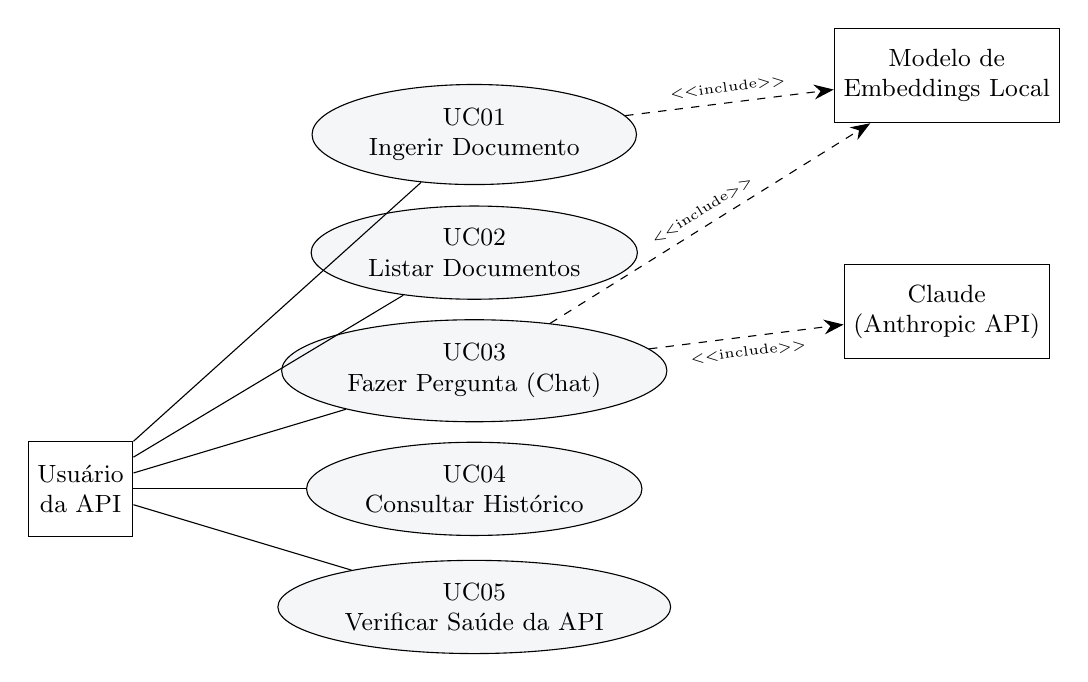
\begin{tikzpicture}[
    ator/.style={draw, minimum height=1.2cm, align=center, font=\small},
    uc/.style={draw, ellipse, minimum width=3.6cm, minimum height=1cm, align=center, font=\small, fill=cinzaclaro},
    linha/.style={draw, -},
    inclui/.style={draw, dashed, -{Stealth[length=2.5mm]}}
]
    \node[ator] (usuario) at (0, -1.5) {Usuário\\da API};

    \node[uc] (uc1) at (5, 3)    {UC01\\Ingerir Documento};
    \node[uc] (uc2) at (5, 1.5)  {UC02\\Listar Documentos};
    \node[uc] (uc3) at (5, 0)    {UC03\\Fazer Pergunta (Chat)};
    \node[uc] (uc4) at (5, -1.5) {UC04\\Consultar Histórico};
    \node[uc] (uc5) at (5, -3)   {UC05\\Verificar Saúde da API};

    \node[ator] (claude) at (11, 0.75) {Claude\\(Anthropic API)};
    \node[ator] (embed) at (11, 3.75)  {Modelo de\\Embeddings Local};

    \draw[linha] (usuario) -- (uc1);
    \draw[linha] (usuario) -- (uc2);
    \draw[linha] (usuario) -- (uc3);
    \draw[linha] (usuario) -- (uc4);
    \draw[linha] (usuario) -- (uc5);

    \draw[inclui] (uc1) -- node[above, sloped, font=\tiny] {<<include>>} (embed);
    \draw[inclui] (uc3) -- node[above, sloped, font=\tiny] {<<include>>} (embed);
    \draw[inclui] (uc3) -- node[below, sloped, font=\tiny] {<<include>>} (claude);
\end{tikzpicture}
\end{center}

\subsection{Especificação dos casos de uso}

\subsubsection{UC01 -- Ingerir Documento}
\textbf{Ator principal:} Usuário da API\quad\textbf{Ator secundário:} Modelo de
Embeddings Local\\
\textbf{Pré-condições:} Nenhuma.\\
\textbf{Fluxo principal:}
\begin{enumerate}[leftmargin=1.2cm]
    \item O usuário envia \texttt{POST /documents} com \texttt{title} e \texttt{text};
    \item O sistema valida o corpo da requisição (RNF01);
    \item O sistema divide o texto em chunks com overlap (RF02);
    \item Para cada chunk, o sistema gera o embedding via modelo local (RF03);
    \item O sistema armazena os chunks embedded no vector store (RF04);
    \item O sistema registra os metadados do documento e retorna \texttt{201 Created}.
\end{enumerate}
\textbf{Fluxos alternativos:} (A1) corpo inválido/texto vazio $\rightarrow$
\texttt{400} (RN01); (A2) falha no modelo de embeddings $\rightarrow$ \texttt{500},
nenhum dado parcial é persistido.\\
\textbf{Pós-condições:} Documento e seus chunks/embeddings persistidos no estado em
memória da aplicação.

\subsubsection{UC02 -- Listar Documentos}
\textbf{Ator principal:} Usuário da API\\
\textbf{Fluxo principal:} \texttt{GET /documents} $\rightarrow$ lista ordenada por
data de criação, com \texttt{id}, \texttt{title}, \texttt{createdAt},
\texttt{chunkCount} (RF05).\\
\textbf{Fluxo alternativo:} Nenhum documento ingerido $\rightarrow$ \texttt{200} com
lista vazia.\\
\textbf{Pós-condições:} Nenhuma (operação de leitura).

\subsubsection{UC03 -- Fazer Pergunta (Chat RAG)}
\textbf{Ator principal:} Usuário da API\quad\textbf{Atores secundários:} Modelo de
Embeddings Local, Claude API (ou motor heurístico)\\
\textbf{Pré-condições:} Nenhuma (funciona mesmo sem documentos ingeridos, RN04).\\
\textbf{Fluxo principal:}
\begin{enumerate}[leftmargin=1.2cm]
    \item O usuário envia \texttt{POST /chat} com \texttt{question};
    \item O sistema valida o corpo da requisição (RNF01);
    \item O sistema gera o embedding da pergunta (RF07);
    \item O sistema busca os \texttt{RETRIEVAL\_TOP\_K} chunks mais similares
          (RF07);
    \item O sistema monta o prompt com o contexto recuperado (RF08);
    \item Com Claude configurado, chama a API do Claude; sem chave, gera resposta
          heurística a partir do chunk mais similar (RF09);
    \item O sistema registra pergunta, resposta e ids dos chunks no histórico
          (RF10);
    \item O sistema retorna \texttt{200 OK} com o item de histórico criado.
\end{enumerate}
\textbf{Fluxos alternativos:} (A1) \texttt{question} vazia $\rightarrow$
\texttt{400}; (A2) sem chave do Claude $\rightarrow$ resposta heurística, mesmo
contrato de saída (RN03); (A3) nenhum documento ingerido $\rightarrow$ contexto
vazio, fluxo continua (RN04); (A4) falha na chamada ao Claude $\rightarrow$
\texttt{500}, nada é adicionado ao histórico.\\
\textbf{Pós-condições:} Novo item adicionado ao histórico.

\subsubsection{UC04 -- Consultar Histórico}
\textbf{Ator principal:} Usuário da API\\
\textbf{Fluxo principal:} \texttt{GET /history} $\rightarrow$ lista de itens, mais
recentes primeiro, limitada a \texttt{HISTORY\_MAX\_ITEMS} (RF11, RF12).\\
\textbf{Fluxo alternativo:} Nenhuma pergunta feita ainda $\rightarrow$ \texttt{200}
com lista vazia.\\
\textbf{Pós-condições:} Nenhuma (operação de leitura).

\subsubsection{UC05 -- Verificar Disponibilidade da API}
\textbf{Ator principal:} Usuário da API (tipicamente uma ferramenta de
monitoramento)\\
\textbf{Fluxo principal:} \texttt{GET /health} $\rightarrow$ \texttt{200 OK} com
\texttt{\{"status": "ok"\}}. Não depende de nenhum recurso externo.

% ================================================================ 4
\section{Arquitetura do Sistema}

\subsection{Visão arquitetural em camadas}

A aplicação segue uma arquitetura em camadas (\emph{layered architecture}),
isolando responsabilidades HTTP, validação, regra de negócio e integrações
externas.

\begin{center}
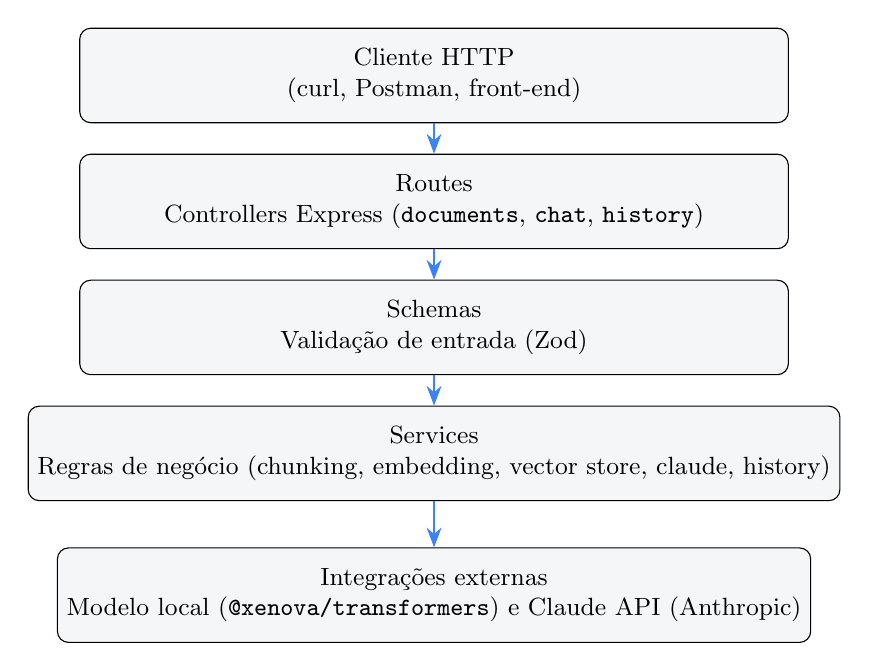
\begin{tikzpicture}[
    camada/.style={draw, rounded corners, minimum width=9cm, minimum height=1.2cm,
                   align=center, font=\small, fill=cinzaclaro},
    seta/.style={-{Stealth[length=2.5mm]}, thick, destaque}
]
    \node[camada] (cliente) at (0,7.6) {Cliente HTTP\\(curl, Postman, front-end)};
    \node[camada] (routes) at (0,6) {Routes\\Controllers Express (\texttt{documents}, \texttt{chat}, \texttt{history})};
    \node[camada] (schemas) at (0,4.4) {Schemas\\Validação de entrada (Zod)};
    \node[camada] (services) at (0,2.8) {Services\\Regras de negócio (chunking, embedding, vector store, claude, history)};
    \node[camada] (externo) at (0,1) {Integrações externas\\Modelo local (\texttt{@xenova/transformers}) e Claude API (Anthropic)};

    \draw[seta] (cliente) -- (routes);
    \draw[seta] (routes) -- (schemas);
    \draw[seta] (schemas) -- (services);
    \draw[seta] (services) -- (externo);
\end{tikzpicture}
\end{center}

Erros de qualquer camada são propagados via \texttt{next(err)} até um middleware
único (\texttt{error-handler.ts}), que decide o status HTTP e o formato da resposta
de erro -- ver ADR-04.

\subsection{Estrutura de diretórios}

\begin{lstlisting}
rag-chat-node/
- src/
  - server.ts              bootstrap do Express + Swagger UI
  - config.ts               leitura de variáveis de ambiente
  - routes/                 documents.route.ts, chat.route.ts, history.route.ts
  - schemas/                documents.schema.ts, chat.schema.ts (Zod)
  - services/               chunking, embedding, vectorStore, document,
                             claude, history, chat
  - middlewares/            error-handler.ts
  - utils/                  cosineSimilarity.ts
  - types/                  index.ts
- tests/                    6 arquivos, 23 testes (unitários + integração)
- openapi.yaml               especificação OpenAPI 3.0
- Dockerfile, docker-compose.yml
\end{lstlisting}

\subsection{Decisões de arquitetura (ADRs)}

\begin{longtable}{p{3.2cm}p{10.3cm}}
\toprule
\textbf{Decisão} & \textbf{Contexto e justificativa} \\
\midrule
\endhead
ADR-01: Vector store em memória (Repository Pattern) &
Escopo de portfólio, não produção com milhões de documentos. Um banco vetorial
externo (Pinecone, Qdrant) adicionaria infraestrutura sem necessidade real neste
volume. \texttt{InMemoryVectorStore} expõe uma interface pequena
(\texttt{add}/\texttt{search}/\texttt{clear}) que isola o resto da aplicação da
estrutura de armazenamento -- trocar por um banco vetorial futuramente significa
reimplementar apenas essa classe. \\
\addlinespace
ADR-02: Motor duplo (Claude + heurístico) &
Uma chave de API paga não deve ser requisito para demonstrar/testar o projeto.
\texttt{claude.service.ts} verifica se \texttt{ANTHROPIC\_API\_KEY} está presente;
sem ela, cai em uma resposta heurística determinística, com o mesmo contrato de
saída (RN03). O projeto fica 100\% demonstrável sem custo e passa a usar IA real
assim que a chave é configurada, sem alteração de código. \\
\addlinespace
ADR-03: Embeddings locais (Lazy Singleton) &
Evita uma segunda dependência de API paga só para vetorização. O modelo
(\texttt{Xenova/all-MiniLM-L6-v2}) roda no próprio processo Node.js via ONNX
runtime; o pipeline é carregado uma única vez (Promise armazenada em módulo),
evitando múltiplas inicializações concorrentes. \\
\addlinespace
ADR-04: Validação centralizada (Zod + middleware único) &
Cada rota declara um schema Zod e delega erros de validação/negócio a um único
\texttt{error-handler}, evitando duplicação de \texttt{try/catch} e garantindo
contrato de erro consistente entre endpoints. \\
\addlinespace
ADR-05: Sem autenticação no MVP &
Escopo do projeto é demonstrar o pipeline RAG, não um sistema multiusuário. Todos
os endpoints são públicos nesta versão -- restrição documentada explicitamente,
não um esquecimento; autenticação por API key seria adicionada como middleware
Express, sem alterar a camada de serviços. \\
\bottomrule
\end{longtable}

\subsection{Diagrama de implantação (Docker)}

\begin{center}
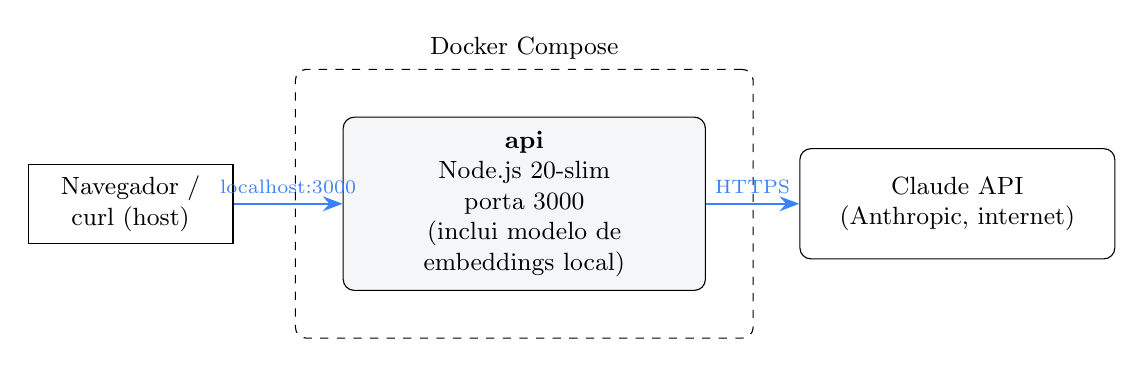
\begin{tikzpicture}[
    container/.style={draw, rounded corners, minimum width=4.6cm, minimum height=2.2cm,
                      align=center, font=\small, fill=cinzaclaro},
    externo/.style={draw, rounded corners, minimum width=4cm, minimum height=1.4cm, align=center, font=\small},
    rede/.style={draw, dashed, rounded corners, inner sep=0.6cm},
    seta/.style={-{Stealth[length=2.5mm]}, thick, destaque}
]
    \node[container] (app) at (0,0) {\textbf{api}\\Node.js 20-slim\\porta 3000\\(inclui modelo de\\embeddings local)};

    \node[rede, fit=(app), label={[font=\small]above:Docker Compose}] {};

    \node[draw, minimum width=2.6cm, minimum height=1cm, align=center, font=\small] (host) at (-5,0) {Navegador /\\curl (host)};
    \node[externo] (claude) at (5.5,0) {Claude API\\(Anthropic, internet)};

    \draw[seta] (host) -- node[above, font=\scriptsize] {localhost:3000} (app);
    \draw[seta] (app) -- node[above, font=\scriptsize] {HTTPS} (claude);
\end{tikzpicture}
\end{center}

A imagem é construída em duas etapas (\emph{multi-stage build}): a etapa
\texttt{build} instala todas as dependências e compila o TypeScript
(\texttt{tsc}); a etapa \texttt{runtime} instala apenas dependências de produção
e copia os artefatos compilados, mantendo a imagem final enxuta. A base é
\texttt{node:20-slim} (Debian/glibc) em vez de Alpine, pois os binários nativos do
\texttt{onnxruntime-node} (usado para embeddings) dependem de glibc e não
funcionam sobre musl. Um volume nomeado persiste o cache do modelo de embeddings
entre reinícios do container, evitando redownload.

% ================================================================ 5
\section{Plano de Testes}
\label{sec:testes}

\subsection{Estratégia de testes}

A estratégia combina dois níveis, ambos com Vitest:

\begin{itemize}[leftmargin=1.5cm]
    \item \textbf{Testes unitários}: módulos determinísticos e puros, sem I/O
          (\texttt{chunking.service}, \texttt{cosineSimilarity},
          \texttt{vectorStore.service}) -- rodam em milissegundos;
    \item \textbf{Testes de integração} (Supertest): endpoints HTTP completos
          sobre a \texttt{app} do Express, exercitando o pipeline real de ponta a
          ponta (chunking $\rightarrow$ embedding local real $\rightarrow$ vector
          store $\rightarrow$ resposta heurística, já que os testes não
          configuram \texttt{ANTHROPIC\_API\_KEY}).
\end{itemize}

Não há mocks do modelo de embeddings: os testes de integração usam o modelo real
\texttt{Xenova/all-MiniLM-L6-v2}, validando o pipeline de ponta a ponta.

\subsection{Casos de teste}

\begin{longtable}{p{4.4cm}p{6.8cm}p{2cm}}
\toprule
\textbf{Arquivo de teste} & \textbf{Cenários cobertos} & \textbf{Tipo} \\
\midrule
\endhead
\texttt{chunking.test.ts} & Texto vazio, texto menor que o chunk, divisão com
    overlap, unicidade de ids, erros de parâmetro inválido (6 casos). & Unitário \\
\addlinespace
\texttt{cosineSimilarity.test.ts} & Vetores idênticos, ortogonais, opostos, com
    norma zero, e de dimensões diferentes (5 casos). & Unitário \\
\addlinespace
\texttt{vectorStore.test.ts} & Armazenar/contar, buscar top-K ordenado por score,
    remover por documento, limpar (4 casos). & Unitário \\
\addlinespace
\texttt{documents.route.test.ts} & \texttt{POST /documents} ingere e retorna
    metadados; \texttt{400} para texto vazio; \texttt{GET /documents} lista (3
    casos). & Integração \\
\addlinespace
\texttt{chat.route.test.ts} & \texttt{POST /chat} responde em modo heurístico;
    \texttt{400} para pergunta vazia; responde mesmo sem documentos ingeridos (3
    casos). & Integração \\
\addlinespace
\texttt{history.route.test.ts} & \texttt{GET /history} vazio inicialmente; ordem
    mais recente primeiro após perguntas (2 casos). & Integração \\
\bottomrule
\end{longtable}

\subsection{Evidência de execução}

Suíte executada localmente com \texttt{npx vitest run}:

\begin{lstlisting}
 RUN  v2.1.9 rag-chat-node

 (pass) tests/chunking.test.ts        (6 tests)
 (pass) tests/vectorStore.test.ts     (4 tests)
 (pass) tests/cosineSimilarity.test.ts (5 tests)
 (pass) tests/documents.route.test.ts (3 tests)
 (pass) tests/chat.route.test.ts      (3 tests)
 (pass) tests/history.route.test.ts   (2 tests)

 Test Files  6 passed (6)
      Tests  23 passed (23)
\end{lstlisting}

Além da suíte automatizada, o fluxo completo foi validado manualmente contra a
imagem Docker real (\texttt{docker build} + \texttt{docker run}, base
\texttt{node:20-slim}): \texttt{GET /health} (200), \texttt{POST /documents}
ingerindo um documento de teste (201, \texttt{chunkCount: 1}), \texttt{POST /chat}
respondendo em modo heurístico com o trecho correto recuperado (200),
\texttt{GET /history} refletindo a interação (200) e \texttt{GET /docs} servindo o
Swagger UI (200) -- confirmando que o pipeline de embeddings local funciona
corretamente dentro do container, não apenas em ambiente de desenvolvimento local.

% ================================================================ 6
\section{Como Executar o Projeto}

\begin{lstlisting}
cd rag-chat-node
cp .env.example .env   # opcional: preencher ANTHROPIC_API_KEY para respostas reais
docker compose up --build
\end{lstlisting}

A API fica disponível em \url{http://localhost:3000}, com documentação interativa
em \url{http://localhost:3000/docs}.

Para rodar a suíte de testes automatizados:

\begin{lstlisting}
cd rag-chat-node
npm install
npm test
\end{lstlisting}

Exemplos de uso via \texttt{curl} estão documentados em
\href{run:../docs/05-documentacao-api.md}{\texttt{docs/05-documentacao-api.md}}.

% ================================================================ 7
\section{Conclusão}

Este documento formalizou o processo de engenharia de software aplicado ao
rag-chat-node, desde o levantamento de requisitos até a arquitetura implementada e
o plano de testes que a valida. O projeto foi desenvolvido como peça de portfólio,
com foco em demonstrar boas práticas replicáveis em contexto profissional:
separação clara de camadas, regras de negócio testáveis e isoladas, um motor duplo
que mantém a aplicação 100\% demonstrável sem custo, documentação de API via
OpenAPI, versionamento seguindo Git Flow com commits convencionais, e
empacotamento reprodutível via Docker.

\end{document}
